\chapter{Wykrywanie anomalii}
\label{chap:OD}

\begingroup
\leftskip4em
\rightskip\leftskip
\noindent
\textbf{Abstrakt} W rozdziale przybliżono teorię, problematykę oraz różnice podejść w detekcji anomalii (obserwacji odstających).
\par
\endgroup

\section{Definicja anomalii (obserwacji odstającej)}
Obserwacje odstające to punkty, które nie odpowiadają wzorcowi w zbiorze danych. Barnett i Lewis definiują obserwację odstającą następująco: ,,Obserwacja odstająca jest to obserwacja, której obecność jest różna od pozostałych obserwacji'' \cite{barnett1984outliers}. Rysunek \ref{fig:anomalia} obrazuje przykład obserwacji odstających (anomalii) dla dwuwymiarowego zbioru danych. Zbiór danych posiada przestrzeń {$N_1$}, większość punktów znajduje się wewnątrz tej przestrzeni. Punkty wystarczająco oddalone od przestrzeni $N_1$: $o_1$, $o_2$, $o_3$ -- sklasyfikowane są jako obserwacje odstające (anomalie).
\begin{figure}[h]
    \centering
    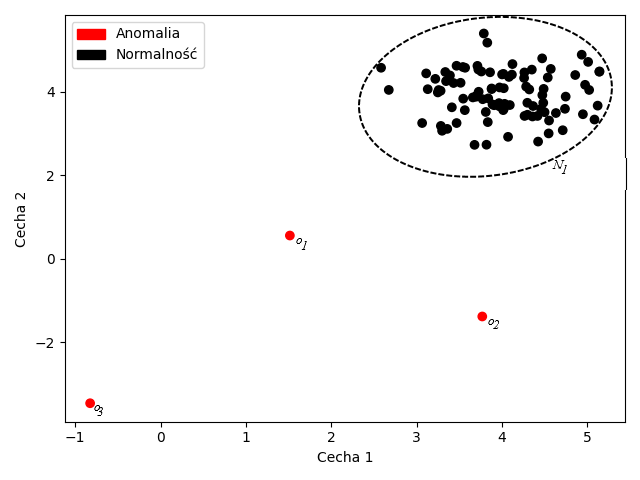
\includegraphics[width=.7\textwidth]{chapters/istniejace/images/anomalia.png}
    \caption{Prosty przykład anomalii w dwuwymiarowym zbiorze danych.}
    \footnotesize{źródło: Opracowanie własne}
    \label{fig:anomalia}
\end{figure}

\section{Zadanie detekcji anomalii}
W pracy rozważamy nienadzorowane zadanie detekcji anomalii na zbiorze $N$ punktów $x_1,...,x_N$ każdy punkt jest d-wymiarowym wektorem liczb rzeczywistych. Zbiór danych składa się z obserwacji poprawnych i anomalnych, jednakże zbiór nie posiada wektora $y_1,..,y_N$ -- klasyfikującego obserwację do obserwacji poprawnych lub anomalnych. Celem zadania detekcji anomalii jest wykrycie punktów anomalnych w danym zbiorze.

\section{Różnice w podejściu detekcji anomalii}

\subsection{Wykrywanie anomalii lokalnych a globalnych}
\label{sub:loc_glob}
Podejście dotyczy wyboru zakresu zbioru jako zbioru odniesienia dla rozpatrywania odstawania danej obserwacji. Główne podejścia to podejście globalne oraz lokalne. Rysunek \ref{fig:anomalie_glob_lok} obrazuje prosty dwuwymiarowy zbiór danych z dwoma klastrami (skupieniami) poprawnych obserwacji: $c_1$ i $c_2$. Dla punktów $x_1 $ oraz $x_2$ klasyfikacja jako anomalie jest możliwa wizualnie. Oba punkty są znacząco oddalone od gęstych obszarów obserwacji. Są to anomalie globalne. Rozpatrując wszystkie obserwacje zbioru punkt $x_3$ mógłby być uznany za poprawną obserwację należącą do klastra $c_2$, jednak kiedy rozpatrzymy podzbiór punktów w sąsiedztwie klastra $c_2$ (zbiór odniesienia), punkt $x_3$ może być uznany za anomalię. Jest to przykład anomalii lokalnej. Zatem anomalia lokalna jest to obserwacja, której odchylenie od normy (anomalność) rozpatrywane jest w obszarze najbliższego sąsiedztwa (zbioru odniesienia). 
\begin{itemize}
    \item Podejście globalne 
    \begin{itemize}
        \item Zbiór odniesienia obejmuje wszystkie obserwacje
        \item Założenie o istnieniu jeden prawidłowego mechanizmu generującego normalne punkty.
        \item Problem: występowanie anomalii lokalnych lub więcej niż jeden prawidłowy mechanizm generujący punkty mogą wypaczyć wynik detekcji
    \end{itemize}
    \item Podejście lokalne 
    \begin{itemize}
        \item Zbiór odniesienia jest podzbiorem całego zbioru
        \item Brak założenia o liczbie mechanizmów generujących.
        \item Problem: wybór odpowiedniego podzbioru jako zbioru odniesienia
    \end{itemize}
\end{itemize}

\begin{figure}[h]
    \centering
    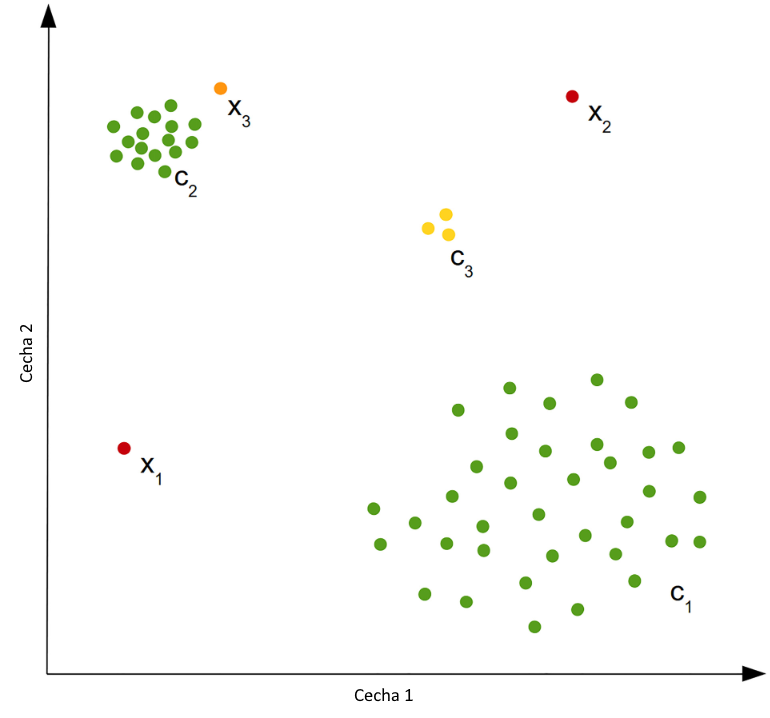
\includegraphics[width=.65\textwidth]{chapters/istniejace/images/mikro_cluste.png}
    \caption{Przykład anomalii globalnych ($x_1, x_2$), lokalnej $x_3$ oraz mikro klastra $c_3$. }
    \footnotesize{źródło: Opracowanie własne na podstawie \cite{goldstein2016comparative}}
    \label{fig:anomalie_glob_lok}
\end{figure}

\subsection{Wynik metody}
\label{sec:score}
Ważnym aspektem dla zadania wykrywania anomalii jest sposób oceny każdej obserwacji. Dane wyjściowe metody mogą przypisywać obserwacji wynik anomalności na dwa warianty:
\begin{itemize}
    \item binarny: przypisanie obserwacji etykiety. Klasyfikacja obserwacji jako anomalii lub poprawnej obserwacji w zbiorze
    \item ciągły: dla każdej obserwacji obliczana jest wartość anomalności np. prawdopodobieństwo obserwacji jako anomalii
\end{itemize}
Podejście przypisujące wynik anomalności w sposób ciągły (wartość anomalności) jest podejściem wszechstronnym. Wykorzystując podejście osoba analizująca dane może za pomocą np. progu wartości anomalności, otrzymać binarną etykietę obserwacji, dostosowując próg dla danej dziedziny.
Wiele podejść opartych na przypisywaniu wyniku anomalności skupia się na wyznaczeniu grupy n-obserwacji o najwyższym wyniku (parametr n często podawany jest przez użytkownika np. procent kontaminacji zbioru danych). 
Podejście oparte na ciągłym wyniku anomalności punktu przydatne jest w rozważaniu mikro klastrów, czyli małych regularnych klastrów. Rysunek \ref{fig:anomalie_glob_lok} obrazuje mikro klaster $c_3$. Algorytm detekcji anomalii powinien przypisać punktom klastra wartość anomalności wyższą od normalnych obserwacji oraz mniejszą od anomalii globalnych. Przykład pokazuje, że podejście przypisywania ciągłej wartości anomalności punktu jest podejściem bardziej użytecznym od binarnej klasyfikacji zwłaszcza w dalszej analizie danych. 

\subsection{Rodzaje anomalii}
% Punktowe, collective i contextual - można wszystko z punktowych które są dominujące w unsupervised detection
W detekcji anomalii wyróżnia się trzy rodzaje anomalii: anomalie punktowe, anomalie zgrupowane oraz anomalie kontekstowe.
Większość dostępnych algorytmów detekcji anomalii dla uczenia nienadzorowanego opiera się na wykrywaniu anomalii punktowych. Detekcja anomalii zgrupowanych została przedstawiona na rysunku \ref{fig:anomalie_glob_lok} i opisana w sekcji \ref{sec:score} -- mikro klaster $c_3$.
Anomalie kontekstowe są to anomalie najczęściej spotykane w szeregach czasowych. Dotyczy to punktów, które mogą być uznane za poprawne obserwacje, jednak rozpatrywane w kontekście charakteru zbioru danych zostaną uznane za anomalie. Weźmy przykład pomiaru temperatury w skali roku we Wrocławiu. Temperatura 25$^{\circ}$C wydaje się poprawnym odczytem temperatury, jednak w kontekście miesiąca np. stycznia. Tak wysoka temperatura jest anomalią.

Szczęśliwie można wykorzystać algorytmy detekcji anomalii punktowych do wykrywania anomalii zgrupowanych i kontekstowych. 
Detekcja różnych typów anomalii wymaga obróbki danych m.in. przekształcenia zbioru danych reprezentującego cechy z wykorzystaniem korelacji, agregacji oraz grupowania \cite{goldstein2014behavior} w celu analizy obserwacji jako anomalii punktowych.

W pracy skupiono się na problemach detekcji anomalii punktowych, wykorzystując bazę zbiorów danych ODDS \cite{ODDS}. Baza zawiera zbiory danych już przygotowanych do zadania detekcji anomalii punktowych.



\section{Główne metodyki detekcji anomalii}
% Dla zadania detekcji anomalii w celu doboru odpowiedniej metody należy na samym początku rozpatrzyć zbiór odniesienia (opisane w podsekcji \ref{sub:loc_glob}) oraz algorytm, który dokładnie modeluje dystrybucję danych. Większość algorytmów detekcji dla uczenia nienadzorowanego opartych jest na następujących metodach:
Dobór metody do detekcji anomalii jest złożonym zadaniem. Detektor anomalii powinien jak najbardziej separować obserwacje odstające od reszty obserwacji. Zdefiniowanie normalnego obszaru zwierającego wszystkie poprawne obserwacje jest ciężkie do osiągnięcia dla rzeczywistych zbiorów danych. Dodatkowo wybrany model powinien zapewnić interpretację wartości anomalności -- dlaczego obserwacja uważana jest za anomalię. Co pozwala na dalszą analizę obserwacji w celu uzyskania informacji na temat jej powstania anomalii oraz znaczenia dla danego zbioru danych. 
\subsection {Metody oparte na wiedzy statystycznej}
Pierwsze metody detekcji anomalii wywodziły się z analizy statystycznej danych. Popularną metodą jest detekcja anomalii z wykorzystaniem rozkład cechy statystycznej. Analizując rozkład cechy statystycznej, wartości znacząco odstające od średniej wartości (regułą trzech sigm) są wartościami odstającymi (anomaliami). Rysunek \ref{fig:pudleko} przedstawia wykres pudełkowy -- sposób wizualizacji rozkładu cechy -- dla którego wartości poza dolnym i górnym wąsem są wartościami odstającymi. 
\begin{figure}[h!]
    \centering
    \includegraphics[width = 0.39\textwidth]{chapters/istniejace/images/wykres-pudełkowy2-1.png}
    \caption{Wykres pudełkowy z wartościami odstającymi}
    \footnotesize{źródło: \cite{pudelko}}
    \label{fig:pudleko}
\end{figure}

    \subsection {Metody oparte na sąsiedztwie obserwacji}
Metody do wyznaczenia wartości anomalności obserwacji rozpatrują sąsiedztwo (zbiór odniesienia) analizowanej obserwacji. Najbardziej popularne podejścia obliczenia anomalności obserwacji względem sąsiedztwa to:
\begin{itemize}
    \item Wykorzystujące klasteryzację: metoda klasteryzuje dane wejściowe na większe i mniejsze skupienia. Wartość anomalności wyznaczana jest z wykorzystaniem odległości obserwacji do najbliższego dużego skupienia oraz rozmiar klastra, do którego przypisano obserwację.
    \item Wykorzystujące metrykę: wartość anomalności obliczana jest jako długość między obserwacją a k najbliższymi sąsiadami. (Przykład opisany w podsekcji \ref{knn})
    \item Wykorzystujące gęstość: wartość anomalności obliczana jest jako stosunek lokalnej gęstości obserwacji do średniej lokalnej gęstości k sąsiadów. (Przykład opisany w podsekcji \ref{lof})
    \item Wykorzystujące miarę kąta: wartość anomalności obliczana jest na podstawie miary kąta między obserwacją a k sąsiadami. Dla wielowymiarowych zbiorów danych miara kąta jest stabilniejszą metryką. (Przykład opisany w podsekcji \ref{abod})
\end{itemize}
\subsection {Metody oparte na łączeniu klasyfikatorów (zespół klasyfikatorów)}
Wykorzystują podejście budowania silnego klasyfikatora składającego się ze słabszych klasyfikatorów. Główne algorytmy korzystające z podejścia to: \textit{Isolation Forest} oraz \textit{Lightweight Online Detector of Anomalies} (LODA). \textit{Isolation Forest} wykorzystuje drzewa decyzyjne do estymacji anomalności obserwacji, natomiast LODA wykorzystuje do tego celu histogramy (algorytmu opisane zostały w podsekcji \ref{iforest} oraz \ref{loda})
\subsection {Metody oparte na sieciach neuronowych}
Podejście wykorzystuje sieci neuronowe do detekcji anomalii. Popularnym rodzajem wykorzystywanych sieci neuronowych są autoenkodery. Jest to jednokierunkowa sieć neuronowe zdolna do rekonstrukcji sygnału wejściowego. Autoenkodery składają się z dwóch elementów: kodera oraz dekodera. Koder przekształca dane wejściowe do niższej wymiarowości, usuwając zbędne informacje, następnie dekoder rekonstruuje dane do wejściowej wymiarowości. Funkcja straty autoenkodera  jest różnicą między danymi wejściowymi a rekonstrukcją danych. Im wyższa funkcja straty tym wyższa anomalność obserwacji.
\begin{figure}
    \centering
    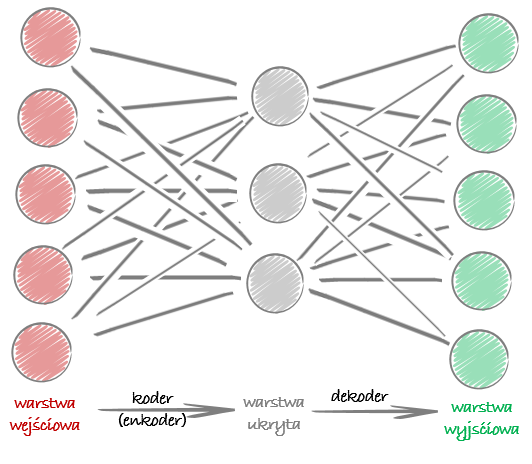
\includegraphics[width = 0.7\textwidth]{chapters/istniejace/images/03-2.png}
    \caption{Budowa autoenkodera}
    \footnotesize{źródło: \cite{ae}}
    \label{fig:pudleko}
\end{figure}

% \section{Proponowane rozwiązanie: MetaOD}
% 
\section{Wykorzystywane algorytmy}
\subsection{ABOD}
\subsection{HBOS}
\subsection{LOF}
\subsection{COF}
\subsection{Isolation Forest}
\subsection{kNN}
\subsection{LODA}
\subsection{OCSVM}
